\documentclass[10pt,journal,compsoc]{IEEEtran}

\ifCLASSOPTIONcompsoc
  \usepackage[compress]{cite}
\else
  % normal IEEE
  \usepackage{cite}
\fi
\usepackage{algorithm}
\usepackage{algpseudocode}
\usepackage{verbatim}
\usepackage{amsmath}
\usepackage{amssymb}
\usepackage{graphicx}
\usepackage{bbm}
\usepackage{listings}
\usepackage{ragged2e}
\usepackage{caption}
\captionsetup[figure]{labelfont={bf},labelformat={default},name={Figure}}




\newtheorem{theorem}{Theorem}[section]
\newtheorem{lemma}[theorem]{Lemma}
\newtheorem{proposition}[theorem]{Proposition}
\newtheorem{corollary}[theorem]{Corollary}
\newenvironment{proof}[1][Proof]{\begin{trivlist}
		\item[\hskip \labelsep {\bfseries #1}]}{\end{trivlist}}
\newenvironment{definition}[1][Definition]{\begin{trivlist}
		\item[\hskip \labelsep {\bfseries #1}]}{\end{trivlist}}
\newenvironment{example}[1][Example]{\begin{trivlist}
		\item[\hskip \labelsep {\bfseries #1}]}{\end{trivlist}}
\newenvironment{remark}[1][Remark]{\begin{trivlist}
		\item[\hskip \labelsep {\bfseries #1}]}{\end{trivlist}}
\newcommand{\qed}{\nobreak \ifvmode \relax \else
	\ifdim\lastskip<1.5em \hskip-\lastskip
	\hskip1.5em plus0em minus0.5em \fi \nobreak
	\vrule height0.75em width0.5em depth0.25em\fi}

\newcommand{\bA}{\mathbf{A}}
\newcommand{\bH}{\mathbf{H}}
\newcommand{\bX}{\mathbf{X}}
\newcommand{\bP}{\mathbf{P}}
\newcommand{\bB}{\mathbf{B}}
\newcommand{\bD}{\mathbf{D}}
\newcommand{\bS}{\mathbf{S}}
\newcommand{\bR}{\mathbf{R}}
\newcommand{\bJ}{\mathbf{J}}
\newcommand{\bLambda}{\mathbf{\Lambda}}

\begin{document}
\title{Joint Embedding of Graphs}
\author{Shangsi Wang,
        Joshua T. Vogelstein,
        Carey E. Priebe
         
\IEEEcompsocitemizethanks{\IEEEcompsocthanksitem Shangsi Wang and Carey Priebe are with the Department of Applied Mathematics and Statistics, Johns Hopkins University. \protect E-mail: swang127@jhu.edu, cep@jhu.edu
\IEEEcompsocthanksitem Joshua Vogelstein is with the Department of Biomedical Engineering and Institute for Computational Medicine, Johns Hopkins University \protect E-mail: jovo@jhu.edu}
%\thanks{Manuscript received April 19, 2005; revised August 26, 2015.}
}


% The paper headers
%\markboth{Journal of \LaTeX\ Class Files,~Vol.~14, No.~8, August~2015}%
%{Shell \MakeLowercase{\textit{et al.}}: Bare Demo of IEEEtran.cls for %Computer Society Journals}



\IEEEtitleabstractindextext{
\justify \begin{abstract} 	
Feature extraction and dimension reduction for networks is critical in a wide variety of domains. Efficiently and accurately learning features for multiple graphs has important applications in statistical inference on graphs. We propose a method to jointly embed multiple undirected graphs. Given a set of graphs, the joint embedding method identifies a linear subspace spanned by rank one symmetric matrices and projects adjacency matrices of graphs into this subspace. The projection coefficients can be treated as features of the graphs. We also propose a random graph model which generalizes classical random graph model and can be used to model multiple graphs. We show through theory and numerical experiments that under the model, the joint embedding method produces estimates of parameters with small errors. Via simulation experiments, we demonstrate that the joint embedding method produces features which lead to state of the art performance in classifying graphs. Applying the joint embedding method to human brain graphs, we find it extract interpretable features that can be used to predict individual composite creativity index.
\end{abstract}

% Note that keywords are not normally used for peerreview papers.
\begin{IEEEkeywords}
graphs, embedding, feature extraction, statistical inference
\end{IEEEkeywords}}


% make the title area
\maketitle


\IEEEdisplaynontitleabstractindextext
\IEEEpeerreviewmaketitle


\IEEEraisesectionheading{\section{Introduction}\label{sec:introduction}}
\noindent \IEEEPARstart{I}n many problems arising in science and engineering, graphs arise naturally as data structure to capture complex relationships between a set of objects. Graphs have been used in various application domains as diverse as social networks\cite{otte2002social}, internet mapping\cite{govindan2000heuristics}, brain connectomics\cite{bullmore2011brain}, political voting networks \cite{ward2011network},  and many others. The graphs are naturally high dimensional objects with complicated topological structure, which makes graph clustering and classification a challenge to traditional machine learning algorithms. Therefore, feature extraction and dimension reduction techniques are helpful in the applications of learning graph data. In this paper, we propose an algorithm to jointly embed multiple graphs into low dimensional space. We demonstrate through theory and experiments that the joint embedding algorithm produces features which lead to state of the art performance for subsequent inference tasks on graphs.  \\

\noindent There exist a few unsupervised approaches to extract features from graphs. First, classical Principal Component Analysis can be applied by treating each edge of a graph as a raw feature\cite{jolliffe2002principal}. This approach produces features which are linear combinations of edges, but it ignores the topological structure of graphs and the features extracted are not easily interpretable. Second, features can be extracted by computing summary topological and label statistics from graphs\cite{li2011graph,park2013anomaly}. These statistics commonly include number of edges, number of triangles, average clustering coefficient, maximum effective eccentricity, etc. In general, it is hard to know what intrinsic statistics to compute \textit{a priori} and computing some statistics can be computationally expensive. Third, many frequent subgraph mining algorithms are developed \cite{jiang2013survey}. For example, the fast frequent subgraph mining algorithm can identify all connected subgraphs that occur in a large fraction of graphs in a graph data set\cite{huan2003efficient}. Finally, spectral feature selection can also be applied to graphs. It treats each graph as a node and constructs an object graph based on a similarity measure. Features are computed through the spectral decomposition of this object graph\cite{zhao2007spectral}. \\

\noindent Adjacency Spectral Embedding (ASE) and Laplacian Eigenmap (LE) are proposed to embed a single graph observation\cite{sussman2012consistent, belkin2003laplacian}. The inference task considered in these papers is learning of the block structure of the graph or clustering vertices. Given a set of graphs $\{G_i=(V_i,E_i)\} _{i=1}^{m}$, ASE and LE need to embed an adjacency matrix or Laplacian matrix of $G_i$ individually, and there is no easy way to combine multiple embeddings. The joint embedding method considers the set of graphs together. It takes a matrix factorization approach to extract features for multiple graphs. The algorithm manages to simultaneously identify a set of rank one matrices and project adjacency matrices into the linear subspace spanned by this set of matrices. The joint embedding can be understood as a generalization of ASE for multiple graphs. We demonstrate through simulation experiments that the joint embedding algorithm extracts features which lead to good performance for a variety of inference tasks. In the next section, we review some random graph models and present a model for generating multiple random graphs. In Section 3, we define the joint embedding of graphs and present an algorithm to compute it. In Section 4, we perform some theoretical analyses of our joint embedding. The theoretical results and real data experiments are explored in Section 5. We conclude the paper with a brief discussion of implications and possible future work.

\section{Setting}
We focus on embedding unweighted and undirected graphs for simplicity, although the joint embedding algorithm works on weighted graphs, and directed graphs with some modifications.  Let $\{G_i=(V_i,E_i)\} _{i=1}^{m}$ be $m$ graphs, each with $n$ vertices, and $\bA _i$ be the adjacency matrix of graph $G_i$. The vertices in these graphs should be matched, which means that all the graphs have a common vertex set $V$. The joint embedding algorithm embeds all $G_i$s simultaneously into $\mathbb{R}^d$ and represents $G_i$  by a vector $\lambda_i \in \mathbb{R}^d$. Before discussing the joint embedding algorithm, we need a random graph model on multiple graphs, on which the theoretical analysis is based. Let us first recall a model on a single graph: Random Dot Product Graph\cite{young2007random}. 

\begin{definition} Random Dot Product Graph (RDPG). Let $F$ be a distribution on a set $\mathcal{X} \in \mathbb{R}^d$ satisfying $x^T y \in [0, 1]$ for all $x, y \in \mathcal{X}$. Let $\bX=[x_1^T,x_2^T,...,x_n^T] \in \mathcal{X}^n$. The notation is $(\bX,\bA) \sim RDPG(F)$, if the $x_i$ are independent and identically distributed according to $F$, and conditioned on $\bX$, the $\bA_{st}$ are independent Bernoulli random variables,
	\[ \bA_{st} \sim Bernoulli(x_s^T x_t). \]
	Alternatively,
	\[ P(\bA|\bX) = \prod_{s<t} (x_s^T x_t) ^{ \bA_{st}} (1-x_s^T x_t)^{1- \bA_{st}}.\]
	Also, define $\bP:=\bX\bX^T$ to be edge probability matrix. When the latent positions $\bX$ is regarded as parameter, the notation becomes $\bA \sim RDPG(\bX)$.
\end{definition}
The RDPG is a convenient model which is designed to capture more complex structures than Stochastic Block Model (introduced below). The RDPG can be further generalized to Latent Position Graph by replacing the inner product by a kernel \cite{tang2013universally}. The Adjacency Spectral Embedding of RDPG adjacency matrix is well studied\cite{sussman2014consistent}. Next, we propose a new random graph model which generalizes the RDPG to multiple graphs.

\begin{definition} Multiple Random Eigen Graphs (MREG). Let $\{h_k\}_{k=1}^{d}$ be a set of norm-1 vectors in $\mathbb{R}^{n}$, and  $F$ be a distribution on a set $\mathcal{X} \in \mathbb{R}^d$,  satisfying $\sum\limits_{k=1}^{d} \lambda [k] h_k  h_k^T \  \in [0, 1]^{n \times n} $ for all $\lambda \in \mathcal{X}$, where $\lambda[k]$ is the $k$th entry of vector $\lambda$. The $m$ pairs $\{(\lambda_i, \bA_i)\}_{i=1}^m$ follow a $d$-dimensional multiple random eigen graphs model, and the notation is
	\[\{(\lambda_i,\bA_i)\}_{i=1}^m \sim MREG(F,h_1,...,h_d),\]
	if $\{\lambda_i\}_{i=1}^m$ is independent and identically distributed according to distribution $F$, and conditioned on $\lambda_i$, the entries of $A_i$ are independent Bernoulli random variables,
	\[ \bA_{i}[s,t] \sim Bernoulli( \sum_{k=1}^{d} \lambda_{i}[k] h_{k} [s] h_{k} [t] ). \]
	$\bP_i:=\sum_{k=1}^{d} \lambda_i [k] h_k  h_k^T$ is defined to be the edge probability matrix for graph $i$. In cases that $\{\lambda_i\}_{i=1}^m$ are of primary interest, they are treated as parameters, and it is said $\{\bA_i\}_{i=1}^{m}$ follows a $m$-graph $d$-dimensional multiple random eigen graphs model with the notation:
	\[\{\bA_i\}_{i=1}^{m} \sim MREG(\lambda_1,...,\lambda_m,h_1,...,h_d).\] 
\end{definition}
Compared to the RDPG model, MREG is designed to model multiple graphs. The vectors $\{h_k\}_{k=1}^{d}$ are shared across graphs; a  $\lambda_i$ is sampled for each graph. On a single graph, they are equivalent if the edge probability matrix is positive semidefinite. In MREG, we allow self loops to happen. This is mainly for theoretical convenience. Next, we introduce another random graph model: Stochastic Block Model \cite{holland1983stochastic}, which generalizes the Erdos-Renyi model \cite{erdds1959random}. SBM is a widely used model to study the community structure of a  graph \cite{karrer2011stochastic, lyzinski2015community}.\\

\begin{definition} Stochastic Block Model (SBM). Let $\pi$ be a prior probability vector for block membership which lies in the unit $K-1$-simplex. Denote by $\tau=(\tau_1,\tau_2,...,\tau_n) \in [K]^n$ the block membership vector, where $\tau$ is a multinomial sequence with probability vector $\pi$.
Denote by $\bB \in [0,1]^{K \times K}$ the block connectivity probability matrix. Suppose $\bA$ is a random adjacency matrix given by,
\[ P(\bA|\tau,\bB)= \prod_{i<j} \bB_{\tau_s,\tau_t}^{\bA_{s,t}} (1-\bB_{\tau_s,\tau_t})^{(1-\bA_{s,t})}\] 
Then, $\bA$ is an adjacency matrix of a $K$-block stochastic block model graph, and the notation is $\bA \sim SBM(\pi,\bB)$. Sometimes, $\tau$ may also be treated as the parameter of interest, in this case the notation is $\bA \sim SBM(\tau,\bB)$.
\end{definition}

\noindent The top panel of Figure \ref{fig:ven} shows the relationships between three random graph models defined above and the Erdos-Renyi (ER) model on $1$ graph. The models considered are those conditioned on latent positions, that is $\tau$, $\bX$ and $\lambda$ in SBM, RDPG and MREG respectively are treated as parameters; furthermore, loops are ignored in MREG. If an adjacency matrix $\bA \sim SBM(\tau,\bB)$ and the block connectivity matrix $\bB$ is positive semidefinite, $\bA$ can also be written as an $RDPG(\bX)$ with $\bX$ having at most $K$ distinct rows. If an adjacency matrix $\bA \sim RDPG(\bX)$, then it is also a $1$-graph $MREG(\lambda_1,h_1,...,h_d)$ with $h_k$ being the normalized $k$th column of $\bX$ and $\lambda_1$ being the vector containing the squared norms of columns of $\bX$. However, a $1$-graph $MREG(\lambda_1,h_1,...,h_d)$ is not necessarily an RDPG graph since $\lambda_1$ could contain negative entries which may result in an indefinite edge probability matrix. \\

\noindent The bottom panel of Figure \ref{fig:ven} shows the relationships between the models on multiple graphs. For ER, SBM  and RDPG, the graphs are sampled i.i.d. with the same parameters. MREG has the flexibility to have $\lambda$ differ across graphs, which leads to a more generalized model for multiple graphs. Actually, it turns out that if $d$ is allowed to be as large as $\frac{n(n+1)}{2}$, MREG can represent any distribution on binary graphs, which includes distributions in which edges are not independent.   
\begin{theorem}
	Given any distribution $\mathcal{F}$ on graphs and a random adjacency matrix $\bA \sim \mathcal{F}$, there exists a dimension  $d$, a distribution $F$ on $\mathbb{R}^d$, and a set of vectors $\{h_k\}_{k=1}^d$, such that $\bA \sim MREG(F,h_1,...,h_d)$.
	\label{thm:rep}
\end{theorem}
Theorem \ref{thm:rep} implies that MREG is really a semi-parametric model, which can capture any distribution on graphs. One can model any set of graphs by MREG with the guarantee that the true distribution is in the model with $d$ being large enough. However, in practice, a smaller $d$ may lead to better inference performance due to reduction in the dimensionality. In the next section, we consider the joint embedding algorithm which can be understood as a parameter estimation procedure for MREG.
\begin{figure}[!htbp]
	\centering
	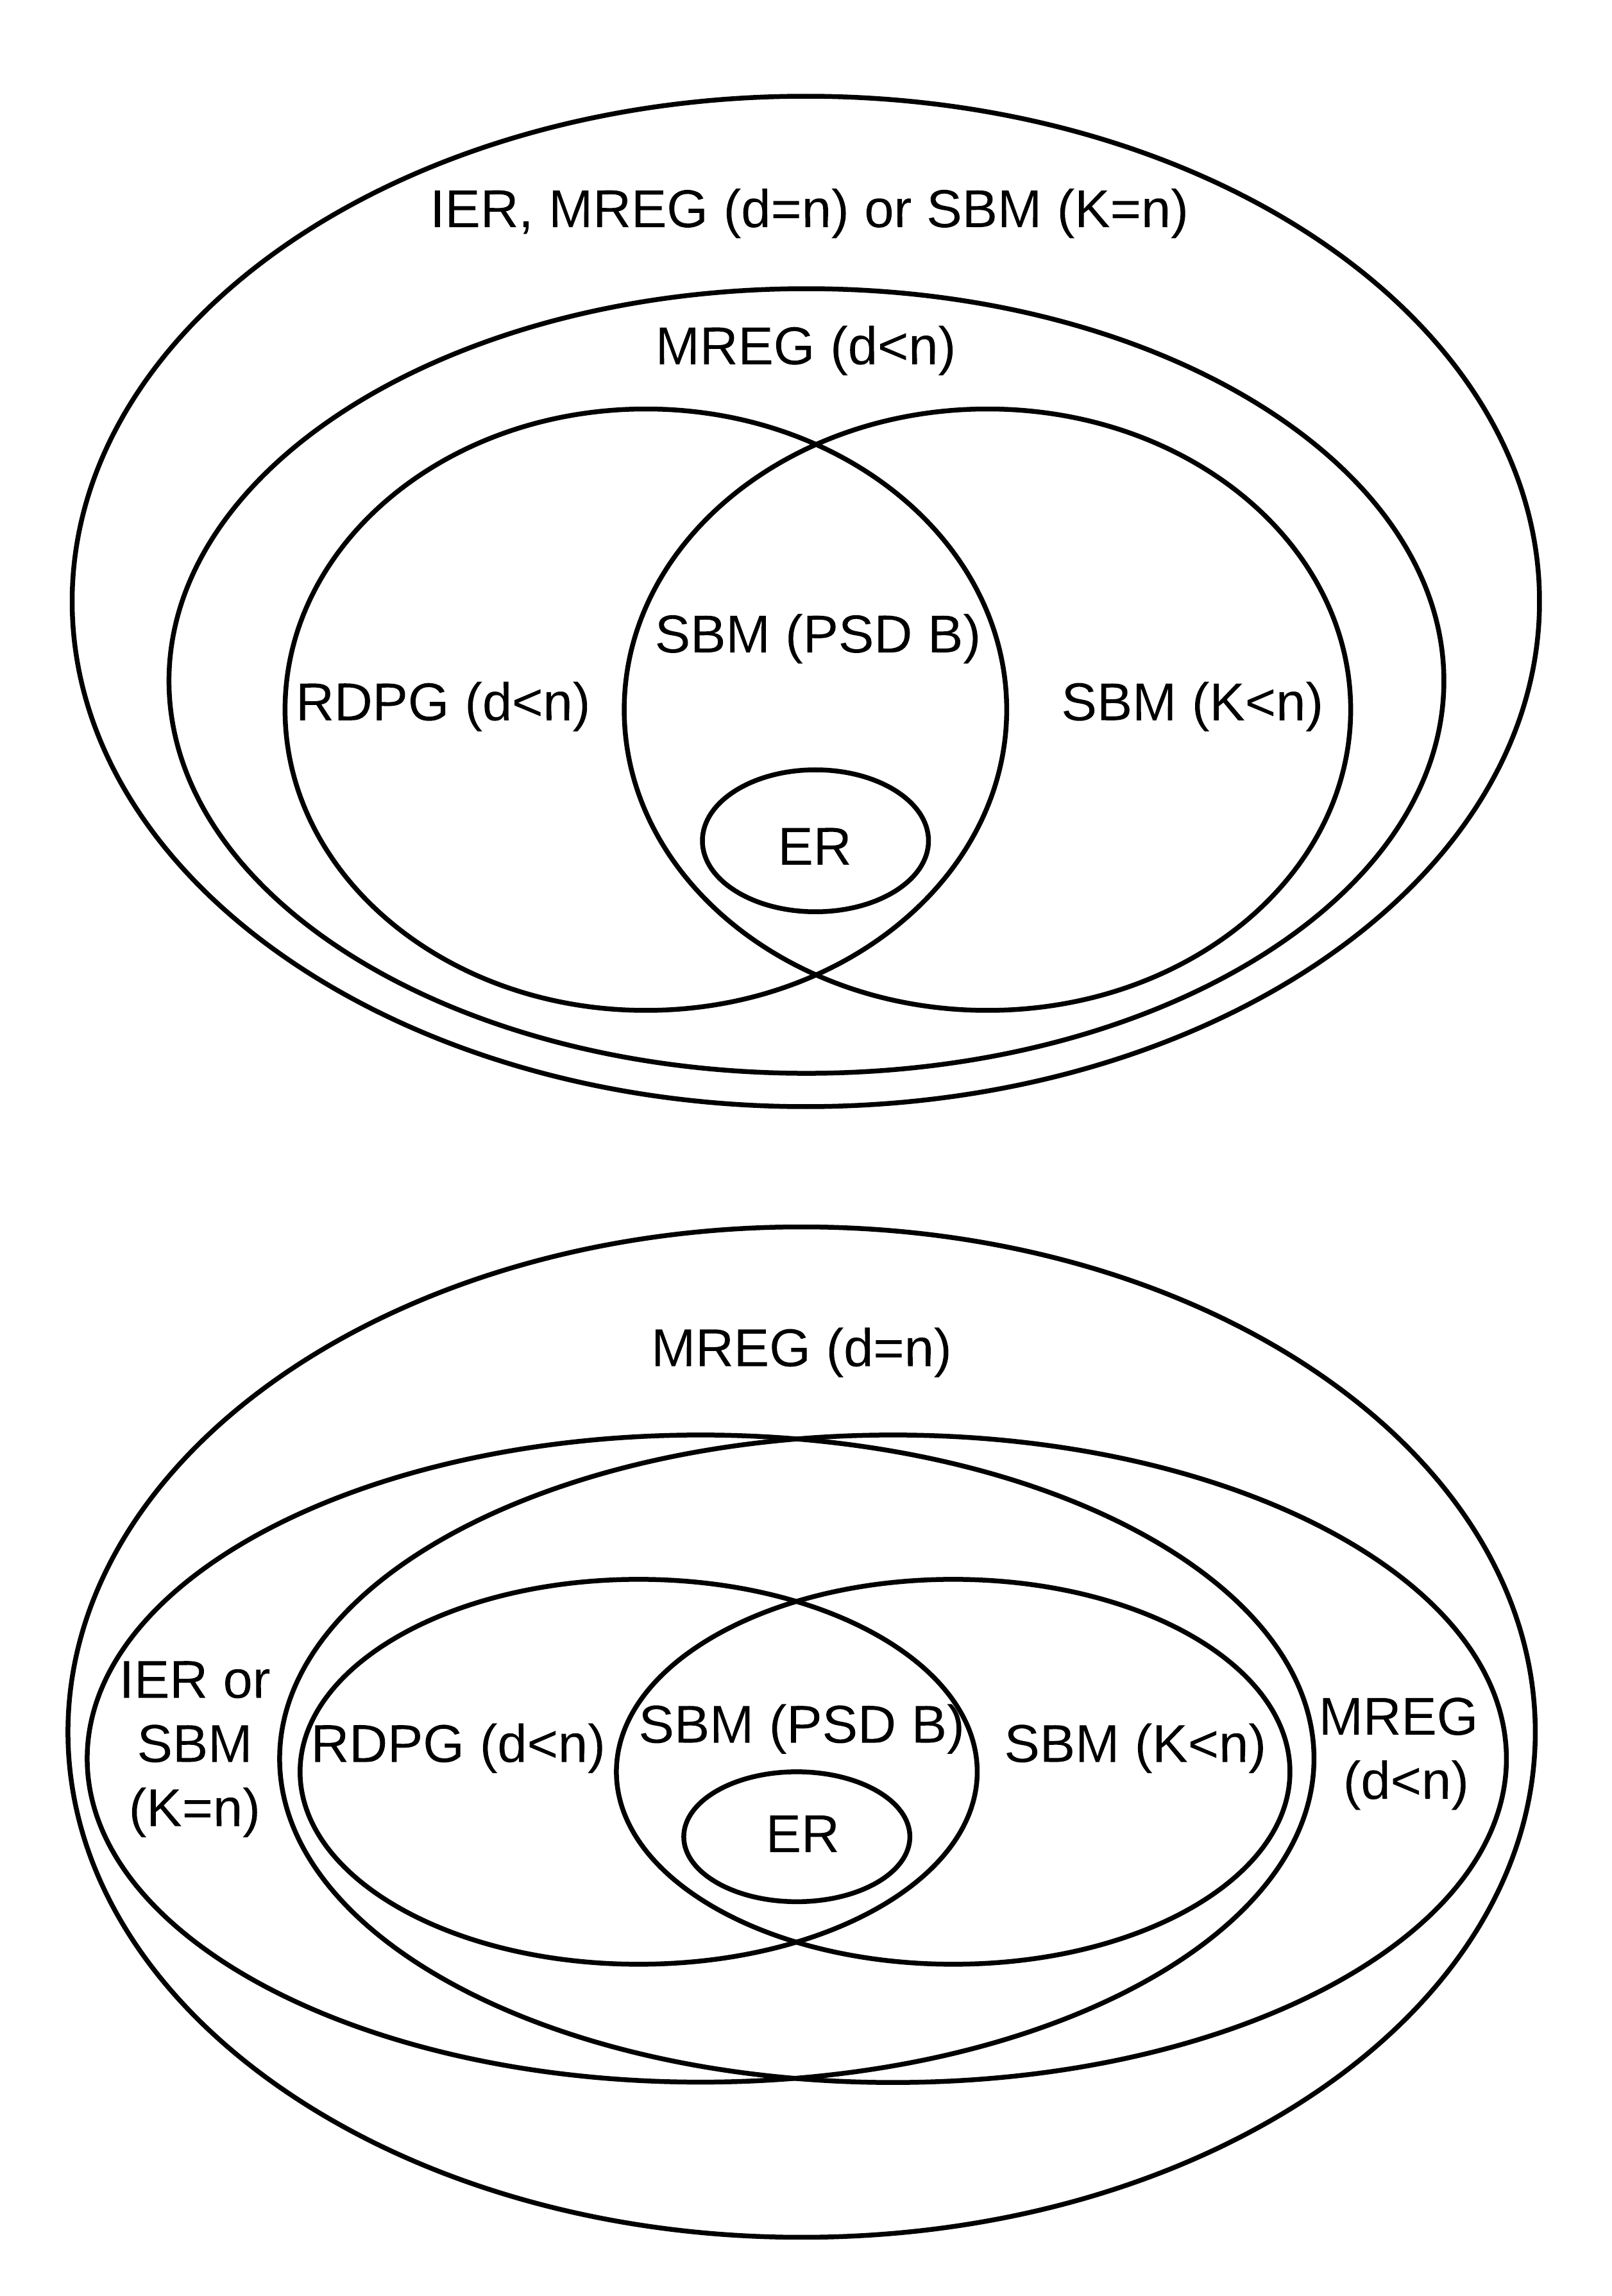
\includegraphics[scale=0.6,width=3.0in]{ven_diag.png}
	\caption{Relationships between random graph models on $1$ graph and multiple graphs. The top panel shows the relationships between the random graph models on $1$ graph. The models considered are those conditioned on latent positions, that is $\tau$, $\bX$ and $\lambda$ in SBM, RDPG and MREG respectively are treated as parameters. ER is a $1$-block SBM. If a graph follows SBM with a positive semidefinite edge probability matrix, it also follows the RDPG model. Any  SBM and  RDPG graph can be represented by a $d$-dimensional MREG model with $d$ being less than or equal to the number of blocks or the dimension of RDPG. On one graph, inhomogeneous ER (IER), $n$-dimensional MREG and $n$-block SBM are equivalent. The bottom panel shows the relationships between the random graph models on multiple graphs. The models considered are those conditioned on latent positions, and for ER, SBM and RDPG graphs are sampled i.i.d. with the same parameters. In this case, MREG has the flexibility to have $\lambda$ differ across graphs, which leads to a more generalized model for multiple graphs.}
	\label{fig:ven}
\end{figure}



\section{Methodology}
\subsection{Joint Embedding of Graphs}
The joint embedding method considers a collection of vertex-aligned graphs, and estimates a common embedding space across all graphs and a loading for each graph. Specifically, it simultaneously identifies a subspace spanned by a set of rank one symmetric matrices and projects each adjacency matrix $\bA_i$ into the subspace. The coefficients obtained by projecting $\bA_i$ are denoted by $\hat{\lambda}_i \in \mathbb{R}^d$, which is called the loading for graph $i$. To estimate rank one symmetric matrices and loadings for graphs, the algorithm minimizes the sum of squared Frobenius distances between adjacency matrices and their projections as described below.
\begin{definition} Joint Embedding of Graphs (JE). Given $m$ graphs $\{G_i \} _{i=1}^{m}$ with $\bA_i$ being the corresponding adjacency matrix, the $d$-dimensional joint embedding of graphs $\{G_i \} _{i=1}^{m}$ is given by
\begin{equation}\label{eq:1}
 (\hat{\lambda}_1,...,\hat{\lambda}_m,\hat{h}_1,...,\hat{h}_d) = \underset{\lambda_i,\|h_k\|=1}{\operatorname{argmin}} \sum\limits_{i=1}^{m} \| \bA_i- \sum\limits_{k=1}^{d} \lambda_{i}[k] h_k h_k^T \|  ^2.  
\end{equation}
Here, $\| \cdot \|$ denotes the Frobenius norm and $\lambda_{i}[k]$ is the $k$th entry of vector $\lambda_i$.
\end{definition}
To make sure that the model is identifiable and avoid the problem scaling, $h_k$ is required to have norm $1$. In addition, $\{h_k h_k^T\}_{k=1}^d$ must be linearly independent to avoid identifiability issue in estimating $\lambda_i$; however, $\{h_k\}_{k=1}^d$ needs not to be linearly independent or orthogonal. To ease the notations, let us introduce two matrices $\bLambda \in \mathbb{R}^{m \times d}$ and $\bH\in \mathbb{R}^{n \times d}$, where $\lambda_i$ is the $i$th row of $\Lambda$ and $h_k$ is the $k$th row of $\bH$; that is, $\bLambda=[\lambda_1^T,...,\lambda_m^T]$ and $\bH=[h_1,...,h_d]$. The equation \eqref{eq:1} can be rewritten using $\bLambda$ and $\bH$ as
\begin{equation*}
(\hat{\bLambda},\hat{\bH}) = \underset{\bLambda,\|h_k\|=1}{\operatorname{argmin}} \sum\limits_{i=1}^{m} \| \bA_i- \sum\limits_{k=1}^{d} \bLambda_{ik} h_k h_k^T \|  ^2.  
\end{equation*}
 Denote the function on the left hand side of the equation by $f(\bLambda,\bH)$ which is explicitly a function of $\lambda_i$s and $h_k$s. There are several alternative ways to formulate the problem. If vector $\lambda_i$ is converted into a diagonal matrix $\bD_i \in \mathbb{R}^{d \times d}$ by putting entries of $\lambda_i$ on the diagonal of $\bD_i$, then solving equation \eqref{eq:1} is equivalent to solving
 \begin{equation*}
\begin{aligned}  
	& \underset{\bD_i,\|h_k\|=1}{\operatorname{argmin}} 
	& & \sum\limits_{i=1}^{m} \| \bA_i- \bH \bD_i \bH^T \|  ^2 \\
	& \text{ subject to} 
	& &  \bD_i \text{ being diagonal.}
\end{aligned}
\end{equation*}
Equation \eqref{eq:1} can be also viewed as a tensor factorization problem. If $\{\bA_i\}_{i=1}^m$ are stacked in a 3-D array ${\mathbb A} \in \mathbb{R}^{m\times n \times n}$, then solving equation \eqref{eq:1} is also equivalent to
\[  \underset{\bLambda,\|h_k\|=1}{\operatorname{argmin}}  \| {\mathbb A} - \sum\limits_{k=1}^{d} \bLambda_{*k} \otimes h_k \otimes h_k\|  ^2,  \]
where $\otimes$ denotes the tensor product and $\bLambda_{*k}$ is the $k$th column of $\bLambda$. \\

\noindent The joint embedding algorithm assumes the graphs are vertex-aligned, unweighted, and undirected. The vertex-aligned graphs are common in applications such as neuroimaging. In case that the graphs are not aligned, graph matching should be performed before the joint embedding \cite{yan2014graduated,park2016encouraging}. The mis-alignments of some vertices definitely have some adverse effects in estimating corresponding latent positions in $H$; however, a small amount of mis-aligned vertices should not have a big impact in estimating $\Lambda$. If the graphs have weighted edges, the joint embedding can still be applied. Also, the MREG model can be easily extended to weighted graphs by replacing the Bernoulli distribution with other proper distributions. In fact, in the experiment of section 5.3, the graphs are weighted, where the edge weights are the log of fiber counts across regions of brains. In case of directed graph, to apply the joint embedding, one can symmetrize the graph by removing the direction of edges. Alternatively, $h_k h_k^T$ in equation \eqref{eq:1} can be replaced by $h_k g_k^T$, with  $h_k$ and $g_k$ representing the in and out latent positions respectively. With this modification, equation \eqref{eq:1} becomes the tensor factorization problem \cite{kolda2009tensor}.\\

\noindent The optimization problem in equation \eqref{eq:1} is similar to Principal Component Analysis (PCA) in the sense of minimizing squared reconstruction error to recover loadings and components \cite{jolliffe2002principal}. However, there are extra symmetries and rank constraints on the components. Specifically, if $h_k h_k^T$ is replaced by a symmetric matrix $\bS_k$ in equation \eqref{eq:1} and $\bS_k$s are required to be orthogonal to each other, then the problem can be solved by applying PCA on vectorized adjacency matrices. The rank constrain can be also viewed as regularization. Compared to PCA, the joint embedding has fewer parameters to estimate, and $h_k$ can be treated as latent positions for vertices, but the joint embedding yields a larger approximation error due to the extra rank constrain. Similar optimization problems have also been considered in the simultaneous diagonalization literature \cite{flury1986algorithm,ziehe2004fast}. The difference is that the joint embedding is estimating an $n$-by-$d$ matrix $\bH$ by minimizing reconstruction error instead of finding a $n$-by-$n$ non-singular matrix by trying to simultaneously diagonalize all matrices. The problem in equation \eqref{eq:1} has considerably fewer parameters to optimize, which makes it more stable and applicable with $n$ being moderately large. In case of embedding only one graph, the joint embedding is equivalent to the Adjacency Spectral Embedding solved by singular value decomposition\cite{sussman2012consistent}. Next, we describe an algorithm to optimize the objective function $f(\bLambda,\bH)$.  

\subsection{Alternating Descent Algorithm}
\noindent The joint embedding of $\{G_i \} _{i=1}^{m}$ is estimated by solving the optimization problem in equation \eqref{eq:1}. There are a few methods proposed to solve similar problems. Carroll and Chang \cite{carroll1970analysis} propose to use an alternating minimization method that ignores symmetry. The hope is that the algorithm will converge to a symmetric solution itself due to symmetry in data. Gradient approaches have also been considered for similar problems \cite{tang2009clustering, kolda2015numerical}. We develop an alternating descent algorithm to minimize $f(\bLambda,\bH)$ that combines ideas from both approaches \cite{bezdek2003convergence}. The algorithm can be also understood as a block coordinate descent method with $\bLambda$ and $\bH$ being the two blocks \cite{wright2015coordinate,beck2013convergence}. The algorithm iteratively updates one of $\bLambda$ and $\bH$ while treating the other parameter as fixed. Optimizing $\bLambda$ when fixing $H$ is straight forward, since it is essentially a least squares problem. However, optimizing $\bH$ when fixing $\bLambda$ is hard due to the fact that the problem is non-convex and there is no closed form solution available. In this case, the joint embedding algorithm utilizes gradient information and take an Armijo backtracking line search strategy to update $\bH$  \cite{nocedal2006numerical}. \\

\noindent Instead of optimizing all columns $\bLambda$ and $\bH$ simultaneously, we consider a greedy algorithm which solves the optimization problem by only considering one column of  $\bLambda$ and $\bH$ at a time. Specifically, the algorithm fixes all estimates for the first $k_0-1$ columns of $\bLambda$ and $\bH$ at iteration $k_0$, and then the objective function is minimized by searching through only the $k_0$th column of $\bLambda$ and $\bH$. That is,
\begin{align}(\hat{\bLambda}_{*k_0},\hat{h}_{k_0}) &= \underset{\bLambda_{*k_0},\|h_{k_0}\|=1}{\operatorname{argmin}} \nonumber\\ &\sum\limits_{i=1}^{m} \| \bA_i- \sum\limits_{k=1}^{k_0-1} \hat{\bLambda}_{ik} \hat{h}_{k} \hat{h}_{k}^T -\bLambda_{ik_0} h_{k_0} h_{k_0}^T\|  ^2.
\label{eq:2}
\end{align} 
Let $f(\bLambda_{*k_0},h_{k_0})$ denote the sum on the left hand side of the equation. To compute a $d$-dimensional joint embedding $(\hat{\bLambda},\hat{\bH})$, the algorithm iteratively solves the one dimensional optimization problem above by letting $k_0$ vary from $1$ to $d$. \\

\noindent There are a few advantages in iteratively solving one dimensional problems. First, there are fewer parameters to fit at each iteration, since the algorithm are only allowed to vary $\bLambda_{*k_0}$ and $h_{k_0}$ at iteration $k_0$. This makes initialization and optimization steps much easier compared to optimizing all columns of $\bH$ simultaneously. Second, it implicitly enforces an ordering on the columns of $\bH$. This ordering allows us to select the top few columns of $\bLambda$ and $\bH$ in cases where model selection is needed after the joint embedding. Third, it allows incremental computation. If $d$ and $d'$ dimensional joint embeddings are both computed, the first $\min(d,d')$ columns of $\hat{\bLambda}$ and $\hat{\bH}$ will be the same. Finally, based on numerical experiments, the difference between optimizing iteratively and optimizing all the parameters when $d$ is small is negligible; however, the iterative algorithm yields a slightly smaller objective function when $d$ is large. The disadvantage of optimizing each column separately is that the algorithm is more likely to end up at a local minimum when the objective function is structured not in favor of embedding iteratively. In practice, this problem can be mitigated by running the joint embedding algorithm several times with random initializations. \\ 

\noindent To find $\bLambda_{*k_0}$ and $h_{k_0}$ in equation \eqref{eq:2}, the algorithm needs to evaluate two derivatives: $\frac{\partial f}{\partial h_{k_0}}$ and $\frac{\partial f}{\partial \bLambda_{i k_0}}$. Denote by $\bR_{ik_0}$ the residual matrix after iteration $k_0-1$ which is $\bA_i- \sum\limits_{k=1}^{k_0-1}\hat{\bLambda}_{ik} \hat{h}_{k} \hat{h}_{k}^T$. The gradient of the objective function with respect to $h_{k_0}$ is given by
\begin{equation} \label{eq:3}
\frac{\partial f}{\partial h_{k_0}} = -4\sum\limits_{i=1}^{m}  \bLambda_{ik_0} (\bR_{ik}-\bLambda_{ik_0} h_{k_0} h_{k_0}^T)  h_{k_0}.
\end{equation}
The derivative of the objective function with respect to $\bLambda_{i k_0}$ is given by
\[\frac{\partial f}{\partial \bLambda_{i k_0}}= -2 \langle \bR_{ik}-\bLambda_{ik_0} h_{k_0} h_{k_0}^T,h_{k_0} h_{k_0}^T\rangle.\]
Setting the derivative to $0$ yields
\begin{equation}  \label{eq:4}
\hat{\bLambda}_{i k_0} = \langle \bR_{ik}, h_{k_0} h_{k_0}^T \rangle,
\end{equation}
where $\langle \cdot , \cdot \rangle$ denotes the inner product. \\

\noindent The joint embedding algorithm alternates between updating $\hat{\bLambda}_{i k_0}$ and $\hat {h}_{k_0}$ according to equation \eqref{eq:3} and \eqref{eq:4}.  Algorithm \ref{alg:je} describes the general procedure to compute the $d$-dimensional joint embedding of graphs $\{G_i\}_{i=1}^m$. The algorithm outputs two matrices: $\hat{\bLambda}$ and $\hat{\bH}$. The rows of $\hat{\bLambda}$ denoted by $\{\hat{\lambda}_i\}_{i=1}^m$ can be treated as estimates of $\{\lambda_i\}_{i=1}^m$ in MREG and features for graphs. Columns of $\hat{\bH}$ denoted by $\{\hat{h}_k\}_{k=1}^d$ are estimates of $\{h_k\}_{k=1}^d$. If a new graph $G$ is observed with adjacency matrix $\bA$, $\bA$ can be projected into the linear space spanned by $\{\hat{h}_k \hat{h}_k^T\}_{k=1}^{d}$ to obtain features for the graph. \\

\noindent In case of $\bA_i$ being large, the updating equations \eqref{eq:3} and \eqref{eq:4} are not practical due to $h_k h_k^T$ and $\bR_{ik}$ being large and dense. However, they can be rearranged to avoid explicit computation of $h_k h_k^T$ and $\bR_{ik}$. The equation \eqref{eq:3} becomes
\begin{align*}
\frac{\partial f}{\partial h_{k_0}} &=-4\sum\limits_{i=1}^{m}  \bLambda_{ik_0} (\bR_{ik}-\bLambda_{ik_0} h_{k_0} h_{k_0}^T)  h_{k_0}\\
&=-4\sum\limits_{i=1}^{m}  \bLambda_{ik_0} \bR_{ik}  h_{k_0} + 4\sum\limits_{i=1}^{m}  \bLambda_{ik_0}^2  h_{k_0} \\
&=-4\sum\limits_{i=1}^{m}  \bLambda_{ik_0} (\bA_i - \sum\limits_{k=1}^{k_0-1} \bLambda_{ik}h_k h_k^T)  h_{k_0} + 4\sum\limits_{i=1}^{m}  \Lambda_{ik_0}^2  h_{k_0} \\
&=-4\sum\limits_{i=1}^{m}  \bLambda_{ik_0} \bA_i h_{k_0} + 4 \sum\limits_{i=1}^{m}  \bLambda_{ik_0} \sum\limits_{k=1}^{k_0-1}  \bLambda_{ik} (h_k^T h_{k_0}) h_k \\
&\qquad {}  + 4\sum\limits_{i=1}^{m}  \bLambda_{ik_0}^2  h_{k_0}.
\end{align*}
Similarly, the equation \eqref{eq:3} can be rewritten as
\begin{align*}  
\hat{\bLambda}_{i k_0} &= \langle \bR_{ik}, h_{k_0} h_{k_0}^T \rangle \\
&=  h_{k_0} ^T \bR_{ik} h_{k_0} \\
&= h_{k_0} ^T (\bA_i - \sum\limits_{k=1}^{k_0-1} \bLambda_{ik}h_k h_k^T) h_{k_0} \\
&= h_{k_0} ^T \bA_i h_{k_0} - \sum\limits_{k=1}^{k_0-1} \bLambda_{ik} (h_{k_0} ^T h_k)^2.
\end{align*}
Based on the rearranged equations, efficiently evaluating matrix vector product $\bA_i h_{k_0}$ is needed to calculate the derivatives. This can be completed for a variety of matrices, in particular, sparse matrices \cite{bell2009implementing}.  \\

\noindent The Algorithm \ref{alg:je} is guaranteed to converge to a stationary point. Specifically, at the termination of iteration $k_0$, $\frac{\partial f}{\partial h_{k_0}} \approx 0$ and $\frac{\partial f}{\partial \bLambda_{i k_0}} \approx 0$. First, $\frac{\partial f}{\partial \bLambda_{i k_0}} \approx 0$ is ensured due to exact updating by equation \eqref{eq:4}. Second notice that updating according to equation \eqref{eq:3} and \eqref{eq:4} always decreases the objective function. Due to the fact that $h_{k_0}$ lies on the unit sphere and the objective is twice continuous differentiable, $\frac{\partial f}{\partial h_{k_0}}$ is Lipschitz continuous. This along with Armijo backtracking line search guarantees a "sufficient" decrease $c\|\frac{\partial f}{\partial h_{k_0}}\|^2$ each time when the algorithm updates $h_{k_0}$ \cite{nocedal2006numerical}, where $c$ is a constant independent of $h_{k_0}$. As a consequence, this implies $\|\frac{\partial f}{\partial h_{k_0}}\| \rightarrow 0$. In general, the objective function may have multiple stationary points due to non-convexity. Therefore, the algorithm is sensitive to initializations. In the experiment below, we initialize $\hat{\bLambda}_{i k_0}$ and $\hat {h}_{k_0}$ through SVD of the average residual matrix $\sum \bR_{ik_0}/m$. When time permits, we recommend running the joint embedding several times with random initializations.\\

\noindent The optimization algorithm described above may not be the fastest approach to solving the problem; however, numerical optimization is not the focus of this paper. Based on results from numerical applications, our approach works well in estimating parameters and extracting features for subsequent statistical inference. Next, we discuss some variations of the joint embedding algorithm.
\begin{algorithm}
	\caption{Joint Embedding Algorithm}
	\label{alg:je}
	\begin{algorithmic}[1]
		\Procedure{Find joint embedding $\hat{\bLambda},\hat{\bH}$ of $\{\bA_i\}_{i=1}^m$}{}
		\State Set residuals: $\bR_{i1}=\bA_i$
		\For{$k=1:d$ }
		\State Initialize $h_k$ and $\bLambda_{*k}$ 
		\While{not convergent}
		\State Fixing $\bLambda_{*k}$, update $h_k$ by gradient descent \eqref{eq:3}
		\State Project $h_k$ back to the unit sphere
		\State Fixing $h_k$, update $\bLambda_{*k}$ by \eqref{eq:4}
		\State Compute objective $\sum\limits_{i=1}^{m} \| \bR_{ik}-  \bLambda_{ik} h_k h_k^T \|^2$
		\EndWhile
		\State Update residuals: $\bR_{i(k+1)}=\bR_{ik}- \bLambda_{ik} h_kh_k^T$
		\EndFor
		\State Output $\hat{\bLambda}=[\bLambda_{*1},...,\bLambda_{*d}]$ and $\hat{\bH}=[h_1,...,h_d]$
		\EndProcedure
	\end{algorithmic}
\end{algorithm}



\subsection{Variations}
The joint embedding algorithm described in the previous section can be modified to accommodate several different settings. \\
\textbf{Variation 1.} When all graphs come from the same distribution, we can force estimated loadings $\hat{\lambda}_i$ to be equal across all graphs. This is useful when the primary inference task is to extract features for vertices. Since all graphs share the same loadings, with slightly abusing notations, let $\bLambda$ be a vector in $\mathbb{R}^d$ and the optimization problem becomes
\[ (\hat{\bLambda},\hat{\bH}) = \underset{\bLambda,\|h_k\|=1}{\operatorname{argmin}} \sum\limits_{i=1}^{m} \| \bA_i- \sum\limits_{k=1}^{d} \bLambda_{k} h_k h_k^T \|  ^2.  \] 
In this case, the optimization problem can be solved exactly by finding the singular value decomposition of the average adjacency matrix $\frac{1}{m}\sum\limits_{i=1}^{m}\bA_i$. \\
\textbf{Variation 2.} When there is a discrete label $y_i \in \mathbb{Y}$ associated with $G_i$ available, we may require all loadings $\hat{\lambda}_i$ to be equal within class. Let $\bLambda \in \mathbb{R}^{|\mathbb{Y}| \times d}$, the optimization problem becomes
\[ (\hat{\bLambda},\hat{\bH}) = \underset{\bLambda,\|h_k\|=1}{\operatorname{argmin}} \sum\limits_{i=1}^{m} \| \bA_i- \sum\limits_{k=1}^{d} \bLambda_{y_i k} h_k h_k ^T \|  ^2.  \] 
In this case, when updating $\bLambda$ as in equation \eqref{eq:4}, the algorithm should average $\bLambda_{y_i k}$ within the same class. \\
\textbf{Variation 3.} In some applications, we may require all $\bLambda_{ik}$ to be greater than $0$, as in non-negative matrix factorization. One advantage of this constraint is that graph $G_i$ may be automatically clustered  based on the largest entry of $\hat{\lambda}_{i}$. In this case, the optimization problem is
\[ (\hat{\bLambda},\hat{\bH}) = \underset{\bLambda \geq 0,\|h_k\|=1}{\operatorname{argmin}} \sum\limits_{i=1}^{m} \| \bA_i- \sum\limits_{k=1}^{d} \bLambda_{ik} h_k h_k ^T \|  ^2.  \] 
To guarantee nonnegativity, the algorithm should use nonnegative least squares in updating $\bLambda$ \cite{kim2008nonnegative}. Furthermore, a constrain on the number of non-zero elements in $i$th row of $\bLambda$ can be added as in K-SVD \cite{aharon2006rm}, and a basis pursuit algorithm should be used to update $\bLambda$ \cite{chen2001atomic, tropp2007signal}. Next, we discuss some theoretical properties of the joint embedding when treated as a parameter estimation procedure for the MREG model.

\section{Theory}
In this section, we consider a simple setting where graphs follow a $1$-dimensional MREG model, that is $\{(\lambda_i,\bA_i)\} _{i=1}^m \sim MREG(F,h_1)$. Under this MREG model, the joint embedding of graphs can be understood as estimators for parameters of the model. Specifically, $\hat{\lambda}_i$ and $\hat{h}_1$ are estimates of $\lambda_i$ and $h$. We prove two theorems concerning the asymptotic behavior of estimator $\hat{h}_1$ produced by joint embedding. \\

\noindent Let $\hat{h}_1^m$ denote the estimates based on $m$ graphs and define functions $\rho$, $D_m$ and $D$ as below: 
\[ \rho(\bA_i,h)= \|\bA_i- \langle \bA_i,h h^T \rangle h h^T\|^2, \]
\[ D_m(h,h_1) =\frac{1}{m}\sum_{i=1}^{m} \rho(\bA_i,h), \]
\[ D(h,h_1) = E(\rho(\bA_i,h)). \]
One can understand $D_m$ and $D$ as sample and population  approximation errors respectively. By equation \eqref{eq:1},
\begin{align*} 
\hat{h}_1^m = \underset{\|h\| =1}{\operatorname{argmin}} \text{ }   \underset{\lambda_i}{\operatorname{argmin}} \sum_{i=1}^{m} \|\bA_i - \lambda_i h h^T\|.
\end{align*}
By equation \eqref{eq:4}, 
\[\langle \bA_i,hh^T \rangle=\underset{\lambda_i}{\operatorname{argmin}} \sum_{i=1}^{m} \|\bA_i - \lambda_i h h^T\|.\]
Therefore,
\[\hat{h}_1^m = \underset{\|h\| =1}{\operatorname{argmin}} \text{ } D_m(h,h_1). \]
The first theorem states that $\hat{h}_1^m$  converges almost surely to the global minimum of $D(h,h_1)$, given that the global minimum is unique. Alternatively, the theorem implies the sample minimizer converges to the population minimizer.
\begin{theorem}
\label{thm:1}
If $D(h,h_1)$ has a unique global minimum at $h'$, then $\hat{h}_1^m$ converges almost surely to $h'$ as $m$ goes to infinity. That is, 
\[ \hat{h}_1^m \overset{a.s.}{\rightarrow} h'. \]
\end{theorem}

\noindent Theorem \ref{thm:1} requires $h'$ to be the unique global minimizer of $D(h,h_1)$. However, the global minimizer is definitely not unique due to the symmetry up to sign flip of $h$, that is $D(h,h_1)=D(-h,h_1)$ for any $h$. This problem can be addressed by forcing an orientation of $\hat{h}_1^m$ or stating that the convergence is up to a sign flip. It is also possible that there are multiple global minimizers of $D(h,h_1)$ which are not sign flips of each other. In this case, Theorem \ref{thm:1} does not apply. We are currently only certain that when all graphs are from the Erdos-Renyi random graph model, the global minimizer is unique up to a sign flip. The next theorem concerns the asymptotic bias of $h'$. It gives a bound on the difference between the population minimizer  $h'$ and the truth $h_1$.

\begin{theorem}
\label{thm:2}
If $h'$ is a minimizer of $D(h,h_1)$, then 
\[\|h'-h_1\| \leq \frac{2 E(\lambda_i)}{E(\lambda_i^2)(h_1^T h')^2}. \]
\end{theorem}

\noindent	To see an application of Theorem \ref{thm:2}, let us consider the case in which all graphs are Erdos-Renyi graphs with $100$ vertices and edge probability of $0.5$. Under this setting, Theorem \ref{thm:2} implies  $\|h'-h_1\| \in [0,0.04] \cup [1.28,1.52]$. The second interval is disturbing. It is due to the fact that when $h_1^T h'$ is small, the bound is useless. We provide some insights as to why the second interval is there and how we can get rid of it with additional assumptions. In the proof of Theorem \ref{thm:2}, we show that the global optimizer $h'$ satisfies
\[h'= \underset{\|h\| =1}{\operatorname{argmax}} \text{ } E(\langle \bA_i,h h^T \rangle ^2). \]
Taking a closer look at $E(\langle \bA_i,h h^T \rangle ^2)$,
\begin{align*}
	E(\langle \bA_i,h h^T \rangle ^2) &= E(\langle \bP_i,h h^T \rangle ^2)+E(\langle \bA_i-\bP_i,h h^T \rangle ^2) \\
	&=E(\lambda_i^2)(h_1^T h)^4+E((h^T (\bA_i-\bP_i)h) ^2).
\end{align*}
Therefore, 
\[h'= \underset{\|h\| =1}{\operatorname{argmax}} \text{ } E(\lambda_i^2)(h_1^T h)^4+E((h^T (\bA_i-\bP_i)h) ^2) .\]
We can see that $E(\lambda_i^2)(h_1^T h)^4$ is maximized when $h=h_1$; however, the noise term $E((h^T (\bA_i-\bP_i)h) ^2)$ is generally not maximized at $h=h_1$. If $n$ is large, we can apply a concentration inequality to $(h^T (\bA_i-\bP_i)h) ^2$ and have an upper bound on $E((h^T (\bA_i-\bP_i)h) ^2)$. If we further assume $A_i$ is not too sparse, that is $E(\lambda_i^2)$ grows with $n$ fast enough, then the sum of these two terms is dominated by the first term. This provides a way to have a lower bound on $h_1^T h'$. We may then replace the denominator of the bound in Theorem \ref{thm:2} by the lower bound. In general, if $n$ is small, the noise term may cause $h'$ to differ from $h_1$ by a significant amount. In this paper, we focus on the case that $n$ is fixed. The case that $n$ goes to infinity for Random Dot Product Graph is considered in \cite{athreya2013limit}.\\


\noindent The two theorems above concern only the estimation of $h_1$, but not $\lambda_i$. Based on equation \eqref{eq:4}, the joint embedding estimates $\lambda_i$ by
\[\hat{\lambda}_i^m= \langle \bA_i,\hat{h}_1^m \hat{h}_1^{m T} \rangle. \]
When $m$ goes to infinity, we can apply Theorem \ref{thm:1},
\[\hat{\lambda}_i^m = \langle \bA_i,\hat{h}_1^m \hat{h}_1^{mT} \rangle \overset{a.s.}{\rightarrow} \langle \bA_i,h' h'^T \rangle = h'^T \bA_i h'.\]
Then, applying the bound on $\|h'-h_1\|$ derived in Theorem \ref{thm:2} and utilizing the fact that $h^T \bA_i h$ is continuous in $h$, we can obtain an upper bound on $|\hat{\lambda}_i^m - h_1^T \bA_i h_1|$. When $\bA_i$ is large, $h_1^T \bA_i h_1$ is concentrated around $\lambda_i$ with high probability. As a consequence, with high probability $|\hat{\lambda}_i^m - \lambda_1|$ is small. In the next section, we demonstrate properties and utilities of the joint embedding algorithm through experiments. 

\section{Experiments}
Before going into details of our experiments, we want to discuss how to select the dimensionality $d$ of the joint embedding. Estimating $d$ is an important model selection question that has been studied for years under various settings \cite{kohavi1995study}. Model selection is not the focus of this paper, but we still face this problem in numerical experiments. In the simulation experiments of this section, we assume $d$ is known to us and simply set the dimensionality estimate $\hat{d}$ equal to $d$. In the real data experiment, we recommend two approaches to determine $\hat{d}$. Both approaches require first running the $d'$-dimensional joint embedding algorithm, where $d'$ is sufficiently large. We then plot the objective function versus dimension, and determine $\hat{d}$ to be where the objective starts to flatten out. Alternatively, we can plot $\{\hat{\bLambda}_{ik}\}_{i=1}^m$ for $k=1,...,d'$, and select $\hat{d}$ when the loadings start to look like noise with $0$ mean. These two approaches should yield a similar dimensionality estimate of $\hat{d}$. 

\subsection{Simulation Experiment 1: Joint Embedding Under a Simple Model}
\noindent In the first experiment, we present a simple numerical example to demonstrate some properties
of the joint embedding procedure as the number of graphs grows. We repeatedly generate graphs with $20$ vertices from $3$-dimensional MREG, where  $\lambda_i[1] \sim \text{Uniform}(8,16)$, $\lambda_i[2] \sim \text{Uniform}(0,4)$ and $\lambda_i[3] \sim \text{Uniform}(0,2)$,  with
\begin{align*}
 h_1 &=[1,1,1,...,1]/\sqrt{20}  \\
 h_2&=[1,-1,1,-1,1,-1,...,-1] /\sqrt{20}  \\
 h_3&=[1,1,-1,-1,1,1,-1,-1,...,-1]/\sqrt{20}. 
\end{align*}
 We keep doubling the number of graphs $m$ from $2^4$ to $2^{12}$. At each value of $m$, we compute the $3$-dimensional joint embedding of graphs. Let the estimated parameters based on $m$ graphs be denoted by $\hat{\lambda}_i^m$ and $\hat{h}_k^m$. Two quantities based on $\hat{h}_k^m$ are calculated. The first is the norm difference between the current $h_k$ estimates and the previous estimates, namely $\|\hat{h}_k^m-\hat{h}_k^{m/2}\|$. This provides numerical evidence for the convergence of our principled estimation procedure. The second quantity is $\|\hat{h}^m_k-h_k\|$. This investigates whether $\hat{h}_k$ is an unbiased estimator for $h_k$. The procedure described above is repeated $20$ times. Figure \ref{fig:db} presents the result. \\
\begin{figure}[!htbp]
	\centering
	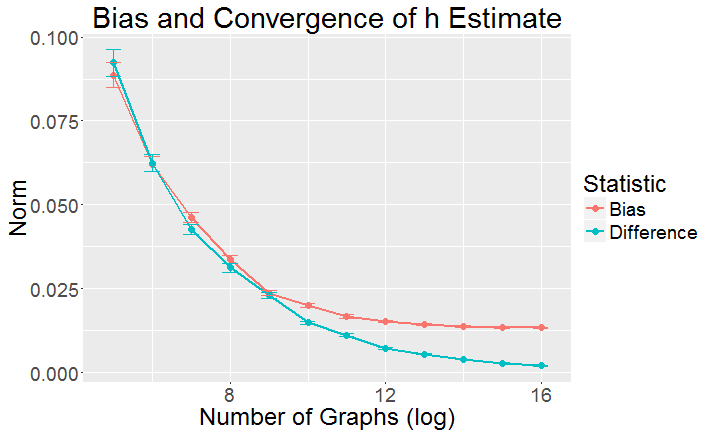
\includegraphics[scale=0.6,width=3.0in]{biasandconv.png}
	\caption{Mean bias ($\|\hat{h}^m_k-h_k\|$) and mean difference between estimates ($\|\hat{h}_k^m-\hat{h}_k^{m/2}\|$) across $20$ simulations are shown. The standard errors are also given by error bars. The graphs are generated from a $3$-dimensional MREG model as described in section 5.1. $\hat{h}_k^m$ has small asymptotic bias; however, it seems to converge as $m$ increases.}
	\label{fig:db}
\end{figure}

\noindent Based on the plot, the norm of differences $\|\hat{h}^m_k-\hat{h}_k^{m/2}\|$ seem to converge to $0$ as $m$ increases. This suggests the convergence of $\hat{h}_1^m$. Second, we notice that the bias $\|\hat{h}^m_2-h_2\|$ and $\|\hat{h}^m_3-h_3\|$ do not converge to $0$; instead, it stops decreasing at around $0.1$ and $0.2$ respectively. This suggests that $\hat{h}_k$ is an asymptotically biased estimator for $h_k$. Actually, this is as to be expected: when there are infinitely many nuisance parameters present, Neyman and Scott demonstrate that maximum likelihood estimator is inconsistent \cite{neyman1948consistent}. In our case, there are infinitely many $\lambda_i$ as $m$ grows; therefore, we do not expect the joint embedding to provide an asymptotic consistent estimate of $h_k$. \\

\noindent In applications such as clustering or classifying multiple graphs, we may be not interested in $\hat{h}_k$. $\hat{\lambda}_i$ is of primary interest, which provides information specifically about the graphs $G_i$. Here, we consider two approaches to estimate $\lambda_i[1]$. The first approach is estimating $\lambda_i[1]$ through joint embedding, that is
\[ \hat{\lambda}_i[1] = \langle \bA_i,  \hat{h}^m_1 \hat{h}^{m T}_1 \rangle. \]
The second approach estimates $\lambda_i$ by assuming $h_1$ is known. In this case, equation \eqref{eq:4} gives 
\[ \hat{\lambda}_i[1] = \langle \bA_i,  h_1 h_1^T \rangle. \]
$\hat{\lambda}_i[1]$ calculated this way can be thought as the 'oracle' estimate. Figure \ref{fig:ld} shows the differences in estimates provided by two approaches. Not surprisingly, the differences are small due to the fact that $\hat{h}_1^m$ and $h_1$ are close.
\begin{figure}[!htbp]
	\centering
	\includegraphics[scale=0.6,width=3.0in]{lambda_diff.png}
	\caption{Distribution of differences between $\hat{\lambda}_i[1]$ estimated using $\hat{h}_1^m$ and $h_1$. The graphs are generated from the $3$-dimensional MREG model as described in section 5.1. The differences are small due to the fact that $\hat{h}_1^m$ and $h_1$ are close.}
	\label{fig:ld}
\end{figure}

\subsection{Simulation Experiment 2: Joint Embedding to Classify Graphs}
In this experiment, we consider the inference task of classifying graphs.  We have $m$ pairs $\{(\bA_i,y_i)\}_{i=1}^{m}$ of observations. Each pair consists of an adjacency matrix $\bA_i \in \{0,1\}^{n \times n}$ and a label $y_i \in [K]$. Furthermore, all pairs are assumed to be independent and identically distributed according to an unknown distribution $\mathbb{F}_{\bA,y}$, that is
\[(\bA_1,y_1),(\bA_2,y_2),...,(\bA_m,y_m) \overset{i.i.d.}{\sim} \mathbb{F}_{A,y}. \] 
The goal is to find a classifier $g$ which is a function $g:\{0,1\}^{n \times n} \rightarrow [K]$ that has a small classification error $L_g=P(g(\bA)\neq y)$. \\ 

\noindent We consider a binary classification problem where $y$ takes value $1$ or $2$. $200$ graphs with $100$ vertices are independently generated. The graphs are sampled from a $2$-dimensional MREG model. Let $h_1$ and $h_2$ be two vectors in $\mathbb{R}^{100}$, and \[h_1=[0.1,...,0.1]^T \text{ , and } h_2=[-0.1,...,-0.1,0.1,...,0.1]^T. \] 
Here, $h_2$ has $-0.1$ as its first $50$ entries and $0.1$ as its last $50$ entries. Gaphs are generated according to the MREG model, 
\begin{equation}
\{(\lambda_i,\bA_i)\}_{i=1}^{200} \sim MREG(F,h_1,h_2),
\label{eq:simu}
\end{equation}
where $F$ is a mixture of two point masses with equal probability, 
\[ F = \frac{1}{2}\mathbb{I} \{\lambda=[25,5]\} + \frac{1}{2}\mathbb{I} \{\lambda=[22.5,2.5]\}.\]
We let the class label $y_i$ indicate which point mass $\lambda_i$ is sampled from. In terms of SBM, this graph generation scheme is equivalent to 
\[ A_i|y_i=1 \sim  SBM((1,...,1,2,...,2),\begin{bmatrix} 0.3 & 0.2 \\ 0.2 & 0.3 \\ \end{bmatrix})  \]
\[ A_i|y_i=2 \sim  SBM((1,...,1,2,...,2),\begin{bmatrix} 0.25 & 0.2 \\ 0.2 & 0.25 \\ \end{bmatrix}).\]

\noindent To classify graphs, we first jointly embed $200$ graphs. The first two dimensional loadings are shown in Figure \ref{fig:load}. We can see two classes are separated after being jointly embedded. 
\begin{figure}[!htbp]
	\centering
	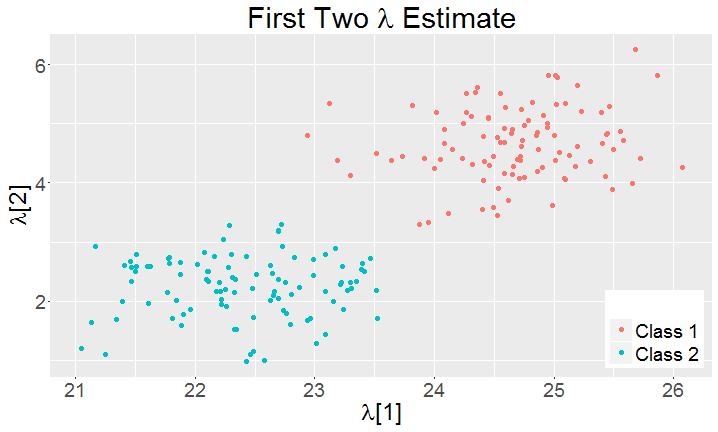
\includegraphics[scale=0.6,width=3.0in]{JE_200.png}
	\caption{Scatter plot of loadings computed by jointly embedding $200$ graphs. The graphs are generated from the $2$-dimensional MREG model as described in equation \eqref{eq:simu}. The loadings of two classes are separated after being jointly embedded. }
	\label{fig:load}
\end{figure}
Then, a $1$-nearest neighbor classifier (1-NN) is constructed based on loadings $\{\hat{\lambda}_i\}_{i=1}^m$.\\

\noindent We compare classification performances of using the joint embedding to extract features to five other feature extraction approaches: Adjacency Spectral Embedding, Laplacian Eigenmap, Graph Statistics, Graph Spectral Statistics, and PCA. For Adjacency Spectral Embedding (ASE) and Laplacian Eigenmap (LE), we first embed each adjacency matrix or normalized Laplacian matrix and then compute the Procrustes distance between embeddings. For Graph Statistics (GS), we compute topological statistics of graphs considered by Park \textit{et al.} in \cite{park2013anomaly}. For Graph Spectral Statistics (GSS), we compute the eigenvalues of adjacency matrices and treat them as features \cite{dorogovtsev2003spectra}. For PCA, we vectorize the adjacency matrices and compute the factors through SVD. After the feature extraction step, we also apply a $1$-NN rule to classify graphs. We let the number of graphs $m$ increase from $4$ to $200$. For each value of $m$, we repeat the simulation $100$ times. Figure \ref{fig:acc} shows the result. The joint embedding takes advantage of increasing sample size and outperforms other approaches when given more than $10$ graphs. 
\begin{figure}[!htbp]
	\centering
	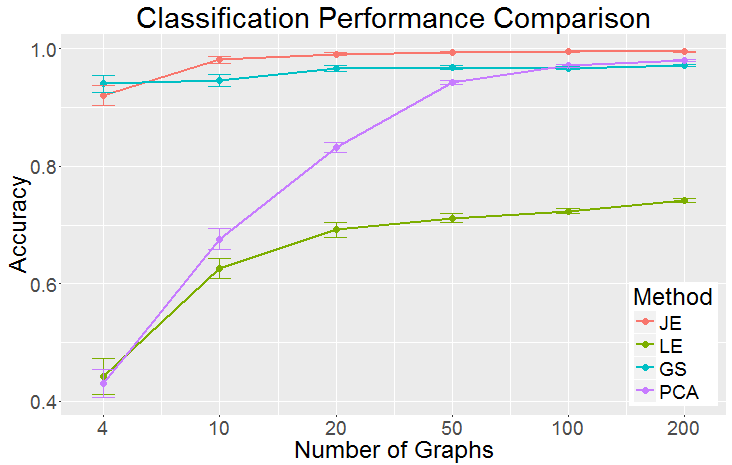
\includegraphics[scale=0.6,width=3.0in]{leig_je_acc.png}
	\caption{Mean classification accuracy of joint embedding, Adjacency Spectral Embedding, Laplacian Eigenmap, Graph Statistics, Graph Spectral Statistics, and PCA with their standard errors are shown. The graphs are generated from a $2$-dimensional MREG model as described in the equation \eqref{eq:simu}. The features are first extracted using methods described above; subsequently, we apply a $1$-NN to classify graphs. For each value of $m$, the simulation is repeated $100$ times. ASE, LE, GS and GSS do not take advantage of increasing sample size in the feature extraction step. PCA has poor performance when the sample sizes is small. Joint embedding takes advantage of increasing sample size and outperforms other approaches when given more than $10$ graphs. }
	\label{fig:acc}
\end{figure} 

\subsection{Real Data Experiment 1: Predict Composite Creativity Index}
In this experiment, we study predicting individual composite creativity index (CCI) through brain connectomes obtained by Multimodal Magnetic Resonance Imaging \cite{koutra2013d}. Neuroimaging and creativity have been jointly investigated previously. Most studies utilize a statistical testing method and find CCI significantly related or inversely related to the activity of some regions of the brain. For a review, please see Arden \textit{et al.} \cite{arden2010neuroimaging}. We embrace a different approach by directly building a prediction model for CCI. First, we jointly embed brain graphs of all subjects. Then, we construct a linear regression model by treating the estimated loadings as explanatory variables and CCI as the response variable. \\

\noindent In total, $113$ healthy, young adult subjects were scanned using a Siemens TrioTim scanner. 3D-MPRAGE and DTI in $35$ directions of the subjects were acquired \cite{brant1992mp}. The images were then registered by Desikan-Killiany Atlas \cite{desikan2006automated}, and a graph of $70$ vertices is constructed. The process of transforming MRI to graphs was completed by NeuroData's MRI Graphs pipeline\cite{kiar2016ndmgcode}. The graphs derived have weighted edges. One example of a graph is shown in the top panel of Figure \ref{fig:cci1}. For each subject, a divergent thinking measure was scored by independent judges using the Consensual Assessment Technique \cite{amabile1983social}, from which the CCI is derived. \\

\noindent To predict the CCI, we first jointly embed $113$ graphs with $d=10$, and then fit a linear model by regressing CCI on $\hat{\lambda}_i$, that is
\[CCI_i \sim \beta_0+\hat{\lambda}_i^T\beta + \epsilon_i. \]
We consider two linear regression models. One using only $\hat{\lambda}_i[1]$ as the explanatory variable, and another one using $\hat{\lambda}_i$ as the explanatory variables. If only the first dimensional loadings are used, the top panel of Figure \ref{fig:cci} shows the result. There is a significant positive linear relationship between CCI and the first dimensional loadings. The first dimensional loadings generally capture the overall connectivity of graphs. In this case, the correlation between the first dimensional loadings and the sum of edge weights is around $0.98$. This model implies that the individual tends to be more creative when there is more brain connectivity. The R-square of this model is $0.07248$, and the model is statistically significantly better when compared to the null model with a p-value $0.0039$, according to the F-test. This model suggests that individual is more creative if the brain is more connected.\\

\noindent If CCI is regressed on the $10$ dimensional loadings, a summary of the linear model is provided in the appendix and a scatter plot of fitted CCI versus true CCI is provided in the bottom panel of Figure \ref{fig:cci}. The R-square is $0.2325$ and the model is statistically significantly better than the null model with a p-value $0.0018$ according to the F-test. It is also significantly better than the model with only $\hat{\lambda}_i[1]$. Although there is still a positive relationship between CCI and the first dimensional loadings, it is no longer significant due to the inclusion of more explanatory variables. In this model, there is a significant negative relationship between CCI and $\hat{\lambda}_i[6]$ based on the t-test. The scatter plot of CCI against $\hat{\lambda}_i[6]$ is given in the middle panel of Figure \ref{fig:cci}. We look into the rank one matrix $\hat{h}_6^T\hat{h}_6$, which is shown in the bottom panel of Figure \ref{fig:cci1}. It has positive connectivity within each hemisphere of the brain, but negative connectivity across hemispheres. This suggests that compared to within-hemisphere connectivity, across-hemisphere connectivity tends to have a more positive impact on human creativity. 

\begin{figure}[!htbp]
	\centering
	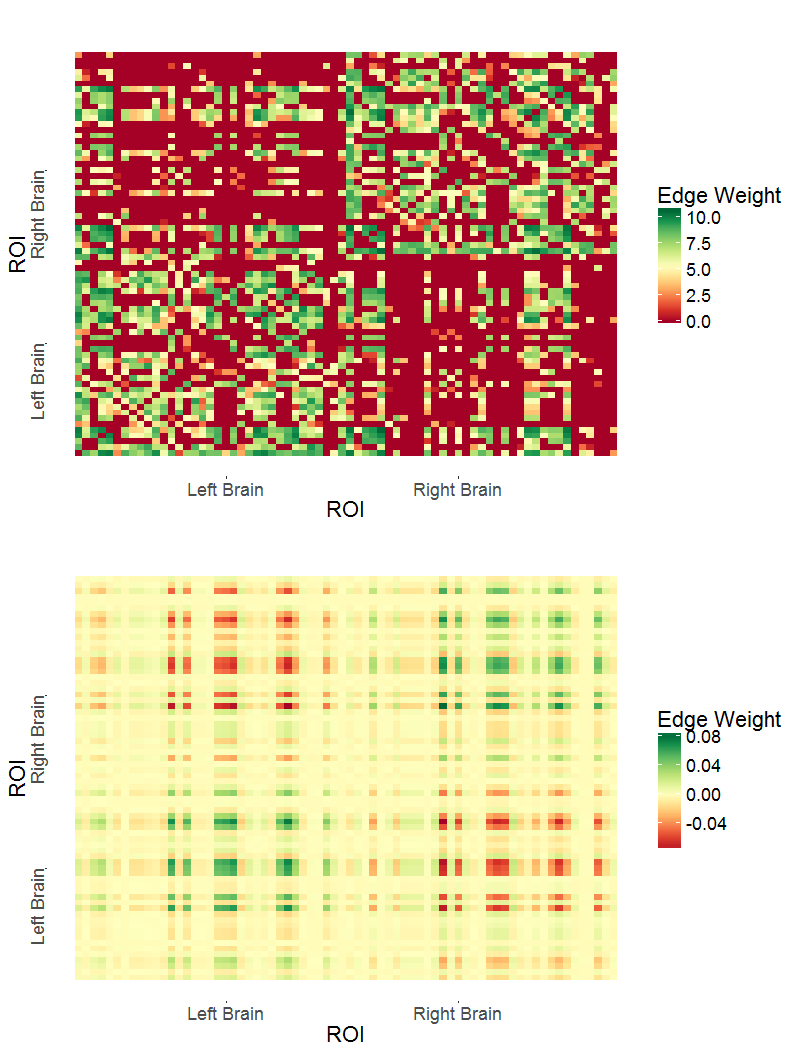
\includegraphics[width=3.0in]{cci_data.png}
	\caption{The top panel shows the graph derived from a typical subject. There is much more neural connectivity within each hemisphere. The bottom panel shows the rank one matrix $\hat{h}_6^T\hat{h}_6$, which has positive  connectivity within each hemisphere, but negative  connectivity across hemispheres.  }
	\label{fig:cci1}
\end{figure} 

\begin{figure}[!htbp]
	\centering
	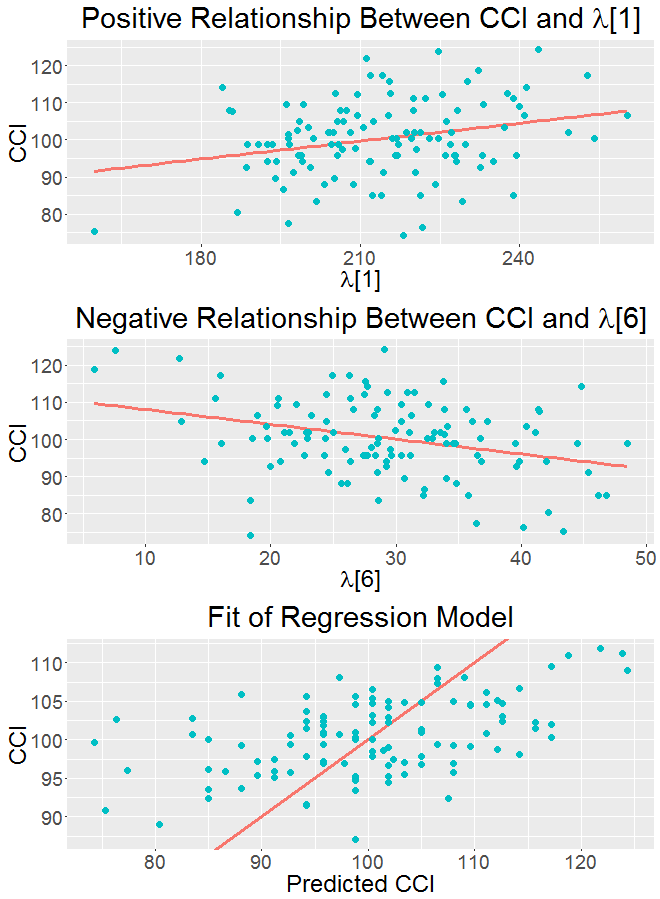
\includegraphics[scale=0.6,width=3.0in]{cci.png}
	\caption{The top panel shows the scatter plot of CCI against $\hat{\lambda}_i[1]$ with the regression line. There is a positive relationship between CCI and first dimensional loadings. The middle panel shows the scatter plot of CCI against $\hat{\lambda}_i[6]$ with regression line. There is a negative relationship between CCI and sixth dimensional loadings. The bottom panel shows the predicted CCI versus true CCI with the identity line.}
	\label{fig:cci}
\end{figure}

\subsection{Real Data Experiment 2: Joint Embedding to Cluster Vertices}
In the previous experiments, we focus on feature extraction for graphs through the joint embedding. Here, we consider a different task, that is spectral clustering through the joint embedding. In general, spectral clustering first computes (generalized) eigenvalues and eigenvectors of adjacency matrix or Laplacian matrix, then clustering the latent positions into groups \cite{sussman2012consistent, belkin2003laplacian}. The cluster identities of latent positions become the cluster identities of vertices of the original graph. When applied to one graph, the joint embedding is equivalent to Adjacency Spectral Embedding (ASE), which is one of the spectral clustering algorithms. When given multiple graphs, the joint embedding can estimate latent positions for graph $i$ as $[\hat{\lambda}_i[1]^{\frac{1}{2}}\hat{h}_1,\hat{\lambda}_i[2]^{\frac{1}{2}}\hat{h}_2,...,\hat{\lambda}_i[d]^{\frac{1}{2}}\hat{h}_d]$ or equivalently $\hat{\bH} \hat{\bD}_i ^ {\frac{1}{2}}$. Then, clustering algorithm can be applied to the latent positions. \\

\noindent We apply the spectral clustering approach to Wikipedia graphs \cite{suwan2016empirical}. The vertices of these graphs represent Wikipedia article pages. The two vertices are connected by an edge if either of the associated pages hyperlinks to the other. Two graphs are constructed based on English webpages and French webpages. The full graph has $1382$ vertices which represents articles within $2$-neighborhood of "Algebraic Geometry".  Based on the content of the associated articles, they are grouped by hand into $6$ categories: People, Places, Dates, Things, Math Terms, and Categories.\\

\noindent We consider a subset vertices  from $3$ categories: People, Things, Math Terms. After taking the induced subgraph of these vertices and removing isolated vertices, there are $n=704$ vertices left. Specifically, $326$, $181$, and $197$ vertices are from People, Things and Math Terms respectively. We consider $4$ approaches to embed the graphs to obtain latent positions: ASE on the English graph (ASE+EN), ASE on the French Graph (ASE+FR), joint embedding on the English graph (JE+EN), and joint embedding on the French Graph (JE+FR). The dimension $d$ is set to $3$ for all approaches, and the latent positions are scaled to have norm $1$ for degree correction. Then, we apply $3$-means to the latent positions. \\ 

\noindent The latent positions of English graph estimated based on the joint embedding is provided in Figure \ref{fig:lp}. The latent positions of Math Terms are separated from the other two clusters. However, the latent positions of People and Things are mixed. Table  \ref{tb:wiki} shows the clustering results measured by adjusted rand index and purity \cite{steinley2004properties,rendon2011internal}. The English graph has clearer community structure than the French Graph. The clustering performance based on latent positions estimated through joint embedding is better. We expect joint embedding to be even better when given more graphs.
\begin{table}[H]
\centering
\begin{tabular}{|l|l|l|l|l|}
	\hline
Method& ASE+EN  & ASE+FR  & JE+EN & JE+FR \\\hline
ARI& 0.147 & 0.115  &{\bf 0.158} & 0.156   \\\hline
Purity& 0.549 & 0.520 &{\bf 0.551} & 0.549 \\
\hline
\end{tabular}
\caption{Clustering Performance on Wikipedia Graphs. The adjusted rand index (ARI) and purity of $4$ spectral clustering approaches are shown. The best result is bolded. The joint embedding estimates latent positions which lead to better clustering performance than ASE.}
\label{tb:wiki}
\end{table}

\begin{figure}[!htbp]
	\centering
	\includegraphics[scale=0.6,width=3.5in]{latent_pos.png}
	\caption{The latent positions of English Graph estimated by the joint embedding are shown. The first three plots on the diagonal are density estimates of latent positions for each dimension and category, and the last plot shows the number of points from each category. The first three plots of the last row show the histogram of latent positions for each dimension and category, and the first three plots of the last column are the corresponding box plot. The pairs plots of latent positions are given in the first three plots below the diagonal, the corresponding correlations are given above the diagonal. The latent positions of Math Terms are separated from the other two clusters. However, the latent positions of People and Things are mixed. }
	\label{fig:lp}
\end{figure}

\section{conclusion}
In summary, we developed a joint embedding method that can simultaneously embed multiple graphs into low dimensional space. The joint embedding can be utilized to estimate features for inference problems on multiple vertex matched graphs. Learning on multiple graphs has significant applications in diverse fields and our results have both theoretical and practical implications for the problem. As the real data experiment illustrates, the joint embedding is a practically viable inference procedure. We also proposed a Multiple Random Eigen Graphs model. It can be understood as a generalization of the Random Dot Product Graph model or the Stochastic Block Model for multiple random graphs. We analyzed the performance of joint embedding on this model under simple settings. We demonstrated that the joint embedding method provides estimates with bounded error. Our approach is intimately related to other matrix and tensor factorization approaches such as singular value decomposition and CP decomposition. Indeed, the joint embedding and these algorithms all try to estimate a low dimensional representation of high dimensional objects through minimizing a reconstruction error. We are currently investigating the utility of joint embedding with more or less regularizations on parameters and under different set ups. We are optimistic that our method provides a viable tool for analyzing multiple graphs and can contribute to a deeper understanding of the joint structure of networks.


%\appendix
\section*{Appendix A}

\begin{proof} [Proof of Theorem 2.1]
 Denote the probability of observing a particular adjacency matrix $\bA_i$ under distribution $\mathcal{F}$ by $p_i$. It suffices to show that there is a set of parameters for MREG such that observing $\bA_i$ under MREG is also $p_i$. \\
 
 \noindent For undirected graphs with loops on $n$ vertices, there are ${n+1}\choose{2}$ possible edges. Let $\bA_1,\bA_2,...,\bA_{2^{{n+1}\choose{2}}}$ be all the possible adjacency matrices. 
 Since real symmetric matrix of size $n$ has ${n+1}\choose{2}$ free entries which lies in a linear space, if there exists ${n+1}\choose{2}$ linearly independent rank one symmetric matrices, they form a basis for this space. It turns out that the rank one symmetric matrices generated by vectors $\{e_i\}_{i=1}^{n} \cup \{e_i+e_j\}_{i<j}$ are linearly independent, where $\{e_i\}_{i=1}^{n}$ is the standard basis for $n$-dimensional Euclidean space. \\
 
 \noindent Next, we construct parameters for the MREG. Let $d$ be ${n+1}\choose{2} $  and 
 \[\{h_k\}_{k=1}^d = \{e_i\}_{i=1}^{n} \cup \{\frac{e_i+e_j}{\sqrt{2}}\}_{i<j}.\] 
 Since $\{h_k h_k^T\}_{k=1}^d$ forms a basis for real symmetric matrices, for each adjacency matrix $\bA_i$, there exists a vector $\lambda_i$, such that 
 \[\bA_i =\sum_{k} \lambda_i [k] h_k  h_k^T.\] Let $F$ be a finite mixture distribution on points $\{\lambda_i\}_{i=1}^{2^{{n+1}\choose{2}}}$, that is 
 \[F = \sum p_i \mathbb{I} \{\lambda = \lambda_i\}.\]
  Under this MREG model, for any adjacency matrix $\bA_i$
 \[P(\bA=\bA_i) = P(\lambda = \lambda_i) = p_i .\]
 This concludes that the distribution $\mathcal{F}$ and $MREG(F,h_1,...,h_d)$ are equal.
 \end{proof}

\begin{proof} [Proof of Theorem 4.1]
First,  we show that $|D_n(h,h_1)-D(h,h_1)|$ converges uniformly to $0$. To begin with, notice three facts:
\begin{itemize}
	\item[(1)] the set $\{h: \|h\|=1\}$ is compact;
	\item[(2)] for all $h$, the function $\rho(\cdot,h)$ is continuous
	\item[(3)] for all $h$, the function $\rho(\cdot,h)$ is bounded by $n^2$.
\end{itemize}
Therefore, by the uniform law of large numbers \cite{jennrich1969asymptotic}, we have
\[\underset{h}{\sup}|D_m(h,h_1)-D(h,h_1)|\overset{a.s.}{\rightarrow} 0.\]
To prove the claim of the theorem, we use a technique similar to that employed by Bickel and Doksum \cite{bickel2015mathematical}. By definition, we must have $D_m(\hat{h}_1^m,h)  \leq D_m(h',h)$ and $D(h',h) \leq D(\hat{h}_1^m,h)$. From these two inequalities,
\begin{align*}
D_m(h',h)-D(h',h) &\geq D_m(\hat{h}_1^m,h)-D(h',h) \\
&\geq D_m(\hat{h}_1^m,h)-D(\hat{h}_1^m,h) .
\end{align*}
Therefore, 
\begin{align*}
|D_m(\hat{h}_1^m,h)-D(h',h)|  \leq  \max(&|D_m(h',h)-D(h',h)|,\\
& |D_m(\hat{h}_1^m,h)-D(\hat{h}_1^m,h)|).
\end{align*}
This implies 
\[ |D_m(\hat{h}_1^m,h)-D(h',h)| \leq \underset{h}{\sup}|D_m(h,h_1)-D(h,h_1)|. \]
Hence, $|D_m(\hat{h}_1^m,h)-D(h',h)|$ must converge almost surely to $0$, that is
\[|D_m(\hat{h}_1^m,h)-D(h',h)|\overset{a.s.}{\rightarrow} 0 .\]
 If $\hat{h}_1^m$ does not converge almost surely to $h'$, then  $\|\hat{h}_1^m-h'\|\geq \epsilon$ for some $\epsilon$ and infinitely many values of $m$. Since $h'$ is the unique global minimum, $|D(\hat{h}_1^m,h)-D(h',h)| > \epsilon' $ for infinitely many values of $m$ and some $\epsilon' $. This contradicts with the previous equation. Therefore, $\hat{h}_1^m$ must converge almost surely to $h'$.
\end{proof}


\begin{proof} [Proof of Theorem 4.2]
The proof of theorem relies on two lemmas. The first lemma shows that
$h'$ is the eigenvector corresponding to the largest eigenvalue of $E(\langle \bA_{i},h' h'^T \rangle \bA_{i})$. The second lemma shows that $E(\langle \bA_{i},h' h'^T \rangle \bA_{i})$ is close to $E(\lambda_i^2) (h_1^Th')^2 h_1 h_1^T$ under Frobenius norm. Then, we apply Davis-Kahan theorem \cite{davis1970rotation} to establish the result of theorem.\\
\begin{lemma}
	The vector $h'$ is the eigenvector corresponding to the largest eigenvalue of $E(\langle \bA_{i},h' h'^T \rangle \bA_{i})$.
\end{lemma}
	We notice that
	\begin{align*}
	\underset{\|h\| =1}{\operatorname{min}}D(h,h_1) &=\underset{\|h\| =1}{\operatorname{min}}E(\|\bA_i- \langle \bA_i,h h^T \rangle h h^T\|^2) \\
	&=\underset{\|h\| =1}{\operatorname{min}}E(\langle \bA_i,\bA_i \rangle- \langle \bA_i,h h^T \rangle ^2) \\
	&=E(\langle \bA_i,\bA_i \rangle)-\underset{\|h\| =1}{\operatorname{max}}E( \langle \bA_i,h h^T \rangle ^2).
	\end{align*}
	Therefore, 
	\begin{equation} \label{eq:5}
	h'= \underset{\|h\| =1}{\operatorname{argmin}} \text{ }D(h,h_1)=\underset{\|h\| =1}{\operatorname{argmax}} \text{ } E(\langle \bA_i,h h^T \rangle ^2) .
	\end{equation}
	Taking the derivative of $E( \langle \bA_i,h h^T \rangle ^2)+ c(h^Th-1)$ with respect to $h$,
	\begin{align*}
	\frac{\partial E( \langle \bA_i,h h^T \rangle ^2)+ c(h^Th-1) }{\partial h} & =  E(\frac{\partial  \langle \bA_i,h h^T \rangle ^2}{\partial h}) +2ch \\
	&=4 E( \langle \bA_i,h h^T \rangle \bA_i)h +2ch .
	\end{align*}
	Setting this expression to $0$ yields,
	\begin{align*} 
	E( \langle \bA_i,h' h'^T \rangle \bA_i)h' & = -\frac{1}{2}ch' .
	\end{align*}
	Using the fact that $\|h'\|=1$, we can solve for $c$:
	\[c = -2 h'^T E( \langle \bA_i,h' h'^T \rangle \bA_i)h' = -2 E( \langle \bA_i,h' h'^T \rangle^2) .\]
	Then, substituting for $c$, 
	\begin{equation}
	E( \langle \bA_i,h' h'^T \rangle \bA_i)h'=E( \langle \bA_i,h' h'^T \rangle^2)h'.
	\end{equation}
	Therefore, we see that $h'$ is an eigenvector of $E(\langle \bA_{i},h' h'^T \rangle \bA_{i})$ and the corresponding eigenvalue is $E(\langle \bA_{i},h' h'^T \rangle ^2)$. Furthermore, $E(\langle \bA_{i},h' h'^T \rangle ^2)$ must be the eigenvalue with the largest magnitude. For if not, then there exists an $h''$ with norm $1$ such that
	\begin{align*}  | h''^T E(\langle \bA_{i},h' h'^T \rangle \bA_{i}) h''| &= |E(\langle \bA_{i},h' h'^T \rangle \langle \bA_{i},h'' h''^T \rangle)| \\
	&> E(\langle \bA_{i},h' h'^T \rangle ^2);
	\end{align*}
	however, by Cauchy-Schwarz inequality we must have
	\begin{align*} E(\langle \bA_{i},h'' h''^T \rangle^2) & E(\langle \bA_{i},h' h'^T \rangle^2) > \\
	&|E(\langle \bA_{i},h' h'^T \rangle \langle \bA_{i},h'' h''^T \rangle)|^2,
	\end{align*}
	implying $E(\langle \bA_{i},h'' h''^T \rangle^2) > E(\langle \bA_{i},h' h'^T \rangle^2)$, which contradicts equation \eqref{eq:5}. Thus, we conclude that $h'$ is the eigenvector corresponding to the largest eigenvalue of $E(\langle \bA_{i},h' h'^T \rangle \bA_{i})$. \\
\begin{lemma}
\[	\|E(\langle \bA_{i},h' h'^T \rangle \bA_{i} ) - E(\lambda_i^2) (h_1^Th')^2 h_1 h_1^T\| \leq 2 E(\lambda_i).\]
\end{lemma}	
	We compute $E(\langle \bA_{i},h' h'^T \rangle \bA_{i})$ by conditioning on $P_i$.
	\begin{align*}
	&E(\langle \bA_{i},h' h'^T \rangle \bA_{i}|\bP_i)    \\
	&=E( \langle \bA_{i}-\bP_i,h' h'^T \rangle (\bA_{i}-\bP_i)|\bP_i)\\
	&\qquad {}+E(\langle \bA_{i}-\bP_i,h' h'^T \rangle \bP_i)|\bP_i) \\
	&\qquad {} +E(\langle \bP_i,h' h'^T \rangle (\bA_{i}-\bP_i)|\bP_i)+E(\langle \bP_i,h' h'^T \rangle \bP_i|\bP_i) \\
	&= E(\langle \bA_{i}-\bP_i,h' h'^T \rangle (\bA_{i}-\bP_i)|\bP_i) + \lambda_i (h_1^Th')^2 \bP_i \\
	&=  2h' h'^T *\bP_i*(\bJ-\bP_i) - DIAG(h_1 h_1^T *\bP_i*(\bJ-\bP_i)) 	\\
	&\qquad {}+\lambda_i (h_1^Th')^2 \bP_i .
	\end{align*}
	Here, DIAG() means only keep the diagonal of the matrix; $*$ means the Hadamard product, and $\bJ$ is a matrix of all ones. Using the fact that $\bP_i=\lambda_i h_1 h_1 ^T$, we have 
	\begin{align*}
	&E(\langle \bA_{i},h' h'^T \rangle \bA_{i}) - E(\lambda_i^2) (h_1^Th')^2 h_1 h_1^T \\
	&=E(E(\langle \bA_{i},h' h'^T \rangle \bA_{i}|\bP_i)-\lambda_i (h_1^Th')^2 \bP_i) 
	 \\
	&= E(2 h' h'^T *\bP_i*(\bJ-\bP_i) \\
	&\qquad {}- DIAG(h' h'^T*\bP_i*(\bJ-\bP_i))).
	\end{align*}
	If we consider the norm difference between $E( \langle \bA_{i},h' h'^T \rangle \bA_{i})$ and $ E(\lambda_i^2) (h_1^Th')^2 h_1 h_1^T$, we have
	\begin{align*}
	&\|E(\langle \bA_{i},h' h'^T \rangle \bA_{i} ) - E(\lambda_i^2) (h_1^Th')^2 h_1 h_1^T\| \\
	&= \|E(2 h' h'^T *\bP_i*(\bJ-\bP_i)  \\
	&\qquad - DIAG(h' h'^T*\bP_i*(\bJ-\bP_i)))\| \\
	&\leq  E(\|2 h' h'^T *\bP_i*(\bJ-\bP_i)  \\
	&\qquad - DIAG(h' h'^T*\bP_i*(\bJ-\bP_i))\|) \\
	&\leq  E(\|2 h' h'^T *\bP_i*(\bJ-\bP_i)\|) \\
	&\leq  E(\|2 h' h'^T * \bP_i\|) \\
	&\leq  2 E(\lambda_i)\| h' h'^T * h_1 h_1^T\| \\
	&=  2 E(\lambda_i) .
	\end{align*}
	This finishes the proof for the lemma. \\
	
	\noindent Notice that the only non-zero eigenvector of $E(\lambda_i^2) (h_1^Th')^2 h_1 h_1^T$ is $h_1$ and the corresponding eigenvalue is $E(\lambda_i^2) (h_1^Th')^2$. We apply the Davis-Kahan theorem \cite{davis1970rotation} to the eigenvector corresponding to the largest eigenvalue of matrices $E(\langle \bA_{i},h' h'^T \rangle \bA_{i} )$ and $E(\lambda_i^2) (h_1^Th')^2 h_1 h_1^T$, yielding
	\[\|h'-h_1\| \leq \frac{2 E(\lambda_i)}{E(\lambda_i^2)(h_1^T h')^2}. \]
	
\end{proof}

\section*{Appendix B}
\noindent{\bf Linear Regression Model Summary}
\begin{lstlisting}
> model<-lm(cci~Lambda+1)
> summary(model)

Call:
lm(formula = cci ~ Lambda + 1)

Residuals:
Min       1Q   Median     3Q    Max 
-26.3432 -6.144 -0.7578 7.1032  16.9004 

Coefficients: Estimate  Pr(>|t|)    
(Intercept)  1.275e+02   0.000275 ***
Lambda1      2.421e-04   0.997981    
Lambda2     -2.326e-01   0.070110 .  
Lambda3     -3.716e-02   0.822592    
Lambda4      8.049e-02   0.687628    
Lambda5     -2.925e-01   0.421858    
Lambda6     -4.285e-01   0.009088 ** 
Lambda7     -1.745e-01   0.590533    
Lambda8     -3.465e-01   0.240093    
Lambda9     -8.970e-01   0.007999 ** 
Lambda10    -8.955e-01   0.052839 .  
---
Signif. codes:  0 ‘***’ 0.001 ‘**’ 
0.01 ‘*’ 0.05 ‘.’ 0.1 ‘ ’ 1

Residual standard error: 9.437 
on 102 degrees of freedom,
Multiple R-squared:  0.2325,
Adjusted R-squared:  0.1572 
F-statistic:  3.09 on 10 and 102 DF,  
p-value: 0.001795
\end{lstlisting}

% references section

% can use a bibliography generated by BibTeX as a .bbl file
% BibTeX documentation can be easily obtained at:
% http://mirror.ctan.org/biblio/bibtex/contrib/doc/
% The IEEEtran BibTeX style support page is at:
% http://www.michaelshell.org/tex/ieeetran/bibtex/
%\bibliographystyle{IEEEtran}
% argument is your BibTeX string definitions and bibliography database(s)
%\bibliography{IEEEabrv,../bib/paper}
%
% <OR> manually copy in the resultant .bbl file
% set second argument of \begin to the number of references
% (used to reserve space for the reference number labels box)



\bibliographystyle{IEEEtran}
\bibliography{citations}

\vspace{-10 mm}
\begin{IEEEbiography}[{\includegraphics[width=1in,height=1.25in,clip,keepaspectratio]{shangsi}}]{Shangsi Wang}
	received the BS degree in mathematics and actuarial science from
	University of Waterloo in 2012, the MA degree from the Department of Applied Mathematics and Statistics at Johns Hopkins University, in 2014.  He is currently a graduate student at the Johns Hopkins University, working toward the PhD degree in statistics. His research interests include statistical inference on random netowrks and pattern recognition in graph datasets.
\end{IEEEbiography}

\begin{IEEEbiography}[{\includegraphics[width=1in,height=1.25in,clip,keepaspectratio]{jovo}}]{Joshua T. Vogelstein}
	received the BS degree from the Department of Biomedical Engineering
	(BME) at Washington University in St. Louis, in 2002, the MS degree from the Department of Applied Mathematics and Statistics at Johns Hopkins University (JHU), in 2009, and the PhD degree from the Department of Neuroscience at JHU in 2009. He was a postdoctoral fellow in AMS at JHU from 2009 until 2011, when he was appointed an assistant research scientist, and became a member of the Institute for Data Intensive Science and Engineering. He spent two years at Information Initiative at Duke, before becoming Assistant Professor in BME at JHU, and core faculty in the Institute for Computational Medicine and the Center for Imaging Science. His research interests include computational statistics, focusing on ultrahigh-dimensional and non-Euclidean neuroscience data, especially connectomics.
\end{IEEEbiography}

\begin{IEEEbiography}[{\includegraphics[width=1in,height=1.25in,clip,keepaspectratio]{carey_priebe}}]{Carey E. Priebe}
	received the BS degree in mathematics from Purdue University, in 1984, the MS degree in computer science from San Diego State University, in 1988, and the PhD 	degree in information technology (computational	statistics) from George Mason University, in 1993. From 1985 to 1994, he worked as a mathematician and scientist in the US Navy research and development laboratory system. Since 1994, he has been a professor in the Department of Applied Mathematics and Statistics, Johns Hopkins University (JHU). His research interests include computational statistics, kernel and mixture estimates, statistical pattern recognition, statistical image analysis, dimensionality reduction, model selection, and statistical inference for high-dimensional and graph data. He is a Senior Member of the IEEE, a Lifetime Member of the Institute of Mathematical Statistics, an Elected Member of the International Statistical Institute, and a Fellow of the American Statistical Association.
\end{IEEEbiography}

% biography section
% 
% If you have an EPS/PDF photo (graphicx package needed) extra braces are
% needed around the contents of the optional argument to biography to prevent
% the LaTeX parser from getting confused when it sees the complicated
% \includegraphics command within an optional argument. (You could create
% your own custom macro containing the \includegraphics command to make things
% simpler here.)

% insert where needed to balance the two columns on the last page with
% biographies
%\newpage




\end{document}



